		\chapter{3D Printing}
        	\index{3D Printing}
			As part of the stage setup there is a \index{winch}winch system - a "reel" and a \index{motors}motor. As the motor turns the string winds up over the reel, and pulls the curtains open.\\
			
			During development I had to rapid prototype this reel. Two options presented themselves - a bolt with nut arrangement, and a 3D printed option.\\
			
			I quickly developed a CAD model for the reel, and sent it off to a friend for printing. I designed the model in \index{Autodesk}Autodesk \index{123D Design}123D Design.\\
			
			\centerline{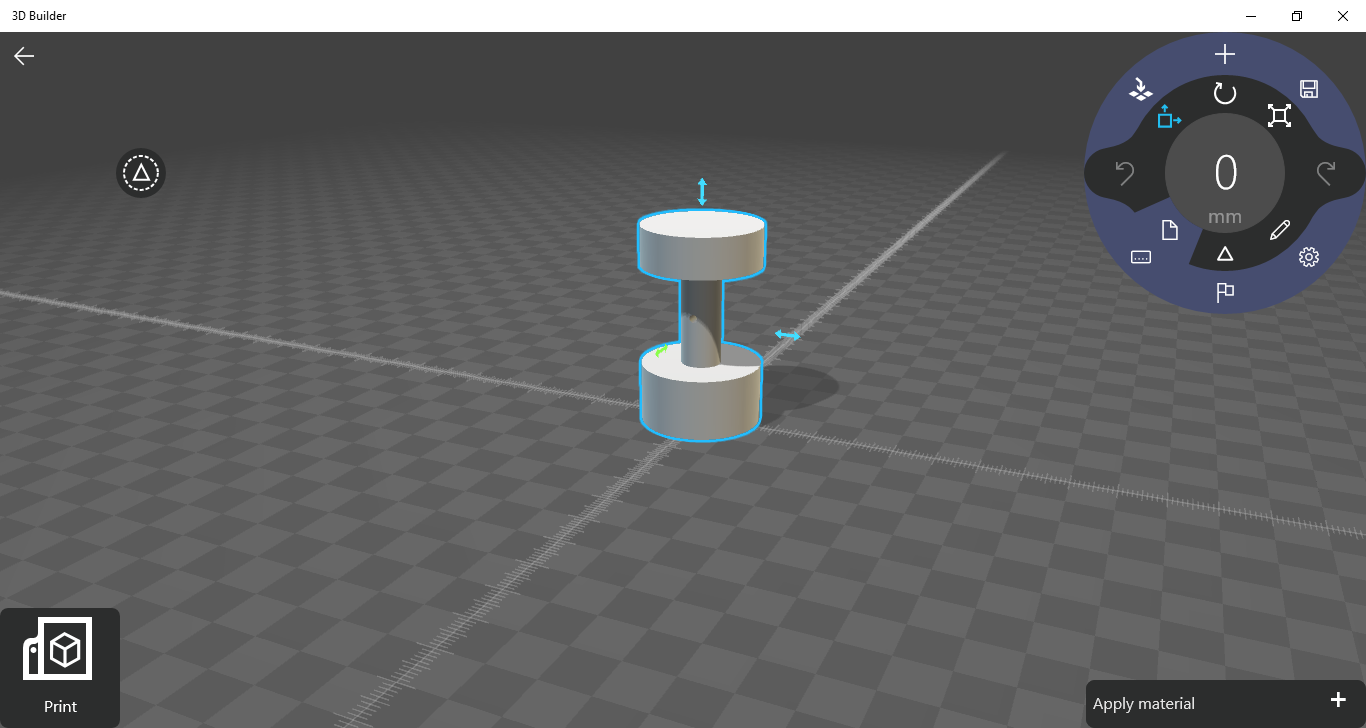
\includegraphics[width=0.75\linewidth]{images/3DPrinting}}
			
			Whilst this was printing I looked around in the box of old robotics parts, and found a wheel hub that I created many years ago. It was a large bolt, with a hole drilled perpendicularly to the shaft into the head of the bolt. It also had a hole drilled down the shaft. The first hole is tapped. This allows the axle of a wheel to be inserted down the shaft, and then a grub inserted into the first hole to hold the axle in place.\\
			
			This also worked, but needed a ridge at the other end of the bolt to stop the string sliding off that way - the most logical option (and the option I took) was to attach a nut to that end. This solution worked great.\\
			
			The 3D model was the first I had made for printing, and I had made one design mistake - that was I made the hole (for the motor axle to fit in) the same size - meaning the axle wouldn't fit in. I've learned my lesson this time though, and know what to do next time. Because of this mistake, I am using the bolt option.\\